\documentclass{article}
\usepackage{graphicx} % Required for inserting images
\usepackage{tikz}
\usetikzlibrary{calc}

\title{12_45}
\author{zhi76.230 }
\date{May 2023}

% \begin{document}

% \maketitle
% https://tex.stackexchange.com/questions/222882/drawing-minimal-xy-axis
% \documentclass[tikz,border=2mm]{standalone}
\begin{document}
% https://tex.stackexchange.com/questions/15994/setting-unit-length-in-tikz
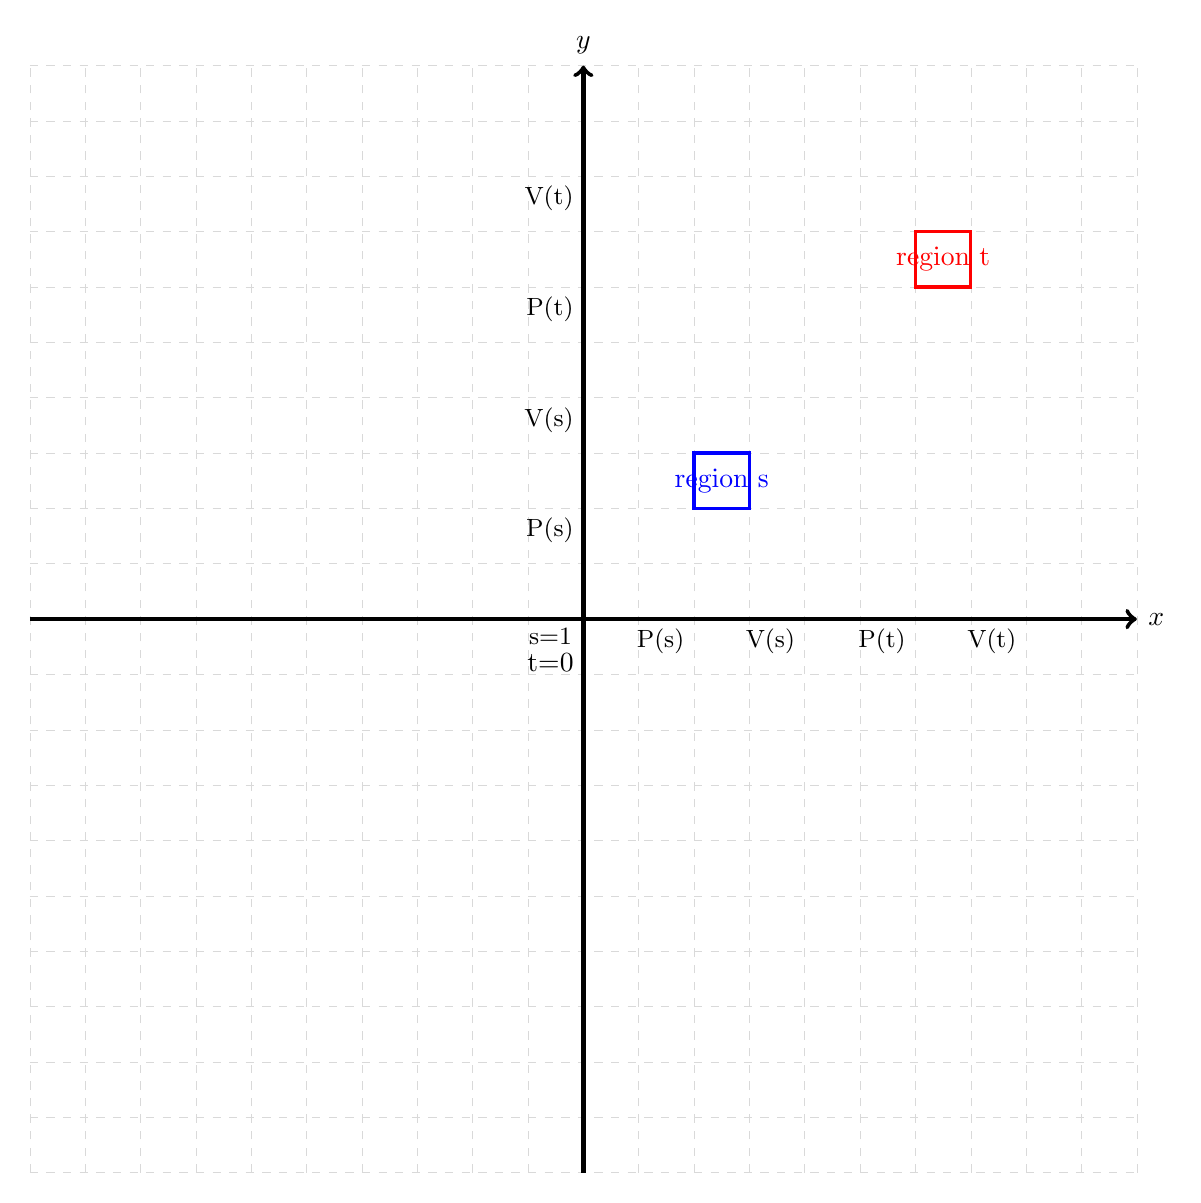
\begin{tikzpicture}[x=20pt,y=20pt]
% https://www.baeldung.com/cs/latex-define-variables
\def\axeswidth{10}
\draw[help lines, color=gray!30, dashed] (-\axeswidth,-\axeswidth) grid[step={($(1, 1) - (0, 0)$)}] (\axeswidth,\axeswidth);
\draw[->,ultra thick] (-\axeswidth,0)--(\axeswidth,0) node[right]{$x$};
\draw[->,ultra thick] (0,-\axeswidth)--(0,\axeswidth) node[above]{$y$};
% https://tex.stackexchange.com/questions/96340/how-to-place-a-textnode-at-the-center-of-a-drawn-rectangle
% https://www.overleaf.com/learn/latex/TikZ_package
% \draw[orange, very thick] (2,2) rectangle (3,3) node[pos=.5] {region k};
\draw[blue, very thick] (2,2) rectangle (3,3) node[pos=.5] {region s};
\draw[red, very thick] (6,6) rectangle (7,7) node[pos=.5] {region t};

% https://tex.stackexchange.com/questions/29233/tikz-adding-text
% https://tikz.dev/tikz-shapes
% https://tex.stackexchange.com/questions/24372/how-to-add-newline-within-node-using-tikz
\node [anchor=north east] at (0,0) {\shortstack{\small s=1\\t=0}};
\node [anchor=north east] at (2,0) {\small P(s)};
\node [anchor=north east] at (4,0) {\small V(s)};
\node [anchor=north east] at (6,0) {\small P(t)};
\node [anchor=north east] at (8,0) {\small V(t)};
\node [anchor=north east] at (0,2) {\small P(s)};
\node [anchor=north east] at (0,4) {\small V(s)};
\node [anchor=north east] at (0,6) {\small P(t)};
\node [anchor=north east] at (0,8) {\small V(t)};
\end{tikzpicture}

\end{document}

% \section{Introduction}

% \end{document}

